\documentclass{minimal}

\usepackage{tikz}
\usetikzlibrary{
	arrows.meta,
	decorations.pathmorphing,
	backgrounds,
	positioning,
	fit,
	petri,
	shapes.misc,
	graphs,
	quotes,
	decorations.pathreplacing,
	calc,
}

%\input{tikz_styles.tex}  % styles used in figures
\tikzset{infectious/.style={
		% The shape:
		rectangle,rounded corners=2mm,
		% The size:
		minimum size=8mm,
		% The border:
		very thick,
		draw=red!50!black!50, % 50% red and 50% black,
		% and that mixed with 50% white
		% The filling:
		top color=white, % a shading that is white at the top...
		bottom color=red!50!black!20, % and something else at the bottom
		% make sure text aligns properly 
		text height=1.5ex,text depth=.25ex,
}}

\tikzset{noninfectious/.style={
		% The shape:
		rectangle,rounded corners=2mm,
		% The size:
		minimum size=8mm,
		% The rest
		very thick,draw=black!50,
		top color=white,bottom color=black!20,
		% make sure text aligns properly 
		text height=1.5ex,text depth=.25ex,
}}

\tikzset{supinfectious/.style={
		% The shape:
		rectangle,rounded corners=2mm,
		% The size:
		minimum size=9.5mm,
		% The border:
		very thick,
		draw=red!50!black!50, % 50% red and 50% black,
		% and that mixed with 50% white
		% The filling:
		top color=white, % a shading that is white at the top...
		bottom color=red!50!black!20, % and something else at the bottom
		% make sure text aligns properly 
		text height=1.5ex,text depth=.25ex,
}}

\tikzset{supnoninfectious/.style={
		% The shape:
		rectangle,rounded corners=2mm,
		% The size:
		minimum size=9.5mm,
		% The rest
		very thick,draw=black!50,
		top color=white,bottom color=black!20,
		% make sure text aligns properly 
		text height=1.5ex,text depth=.25ex,
}}

\begin{document}
	
\pagestyle{empty}

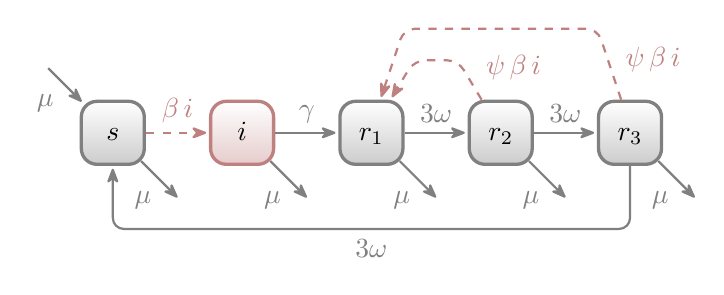
\begin{tikzpicture}[>={Stealth[round]},thick,black!50,text=black,
	every new ->/.style={shorten >=1pt},
	graphs/every graph/.style={edges=rounded corners}]
	\graph [grow right sep=8mm, branch down=7mm] {
		%b [coordinate,xshift=4mm,yshift=7mm] {""} ->[black!50,shorten >=-1.5pt,"$\mu$"]
		s/"$s$" [noninfectious] {"$s$"} ->[dashed,red!50!black!50,"$\beta\,i$"]
		i/"$i$" [infectious] {"$i$"} ->[black!50,"$\gamma$"]
		r1/"$r_1$" [noninfectious] {"$r_1$"} ->[black!50,"$3\omega$"]
		r2/"$r_2$" [noninfectious] {"$r_2$"} ->[black!50,"$3\omega$"]
		r3/"$r_3$" [noninfectious] {"$r_3$"};
	};
		\draw [->,rounded corners,shorten >= 1pt] ($(r3.south)$) -- ($ (r3.south) + (0mm,-8mm) $) to [edge label=$3\omega$,color=black!50] ($ (s.south) + (0mm,-8mm) $) -- ($ (s.south) $);
		\draw [->,rounded corners,shorten >= 1pt,dashed,red!50!black!50,] ($(r2.120)$) to [edge label'=$\psi\,\beta\,i$,color=red!50!black!50,%yshift=-2.5mm
		] ($ (r2.120) + (-1.5mm,2.5mm) $) -- ($ (r2.120) + (-3mm,5mm) $) -- ($ (r1.60) + (3mm,5mm) $) -- ($ (r1.60) $);
		\draw [->,rounded corners,shorten >= 1pt,dashed,red!50!black!50,] ($(r3.105)$) to [edge label'=$\psi\,\beta\,i$,color=red!50!black!50] ($ (r3.105) + (-1.5mm,4.5mm) $) -- ($ (r3.105) + (-3mm,9mm) $) -- ($ (r1.75) + (3mm,9mm) $) -- ($ (r1.75) $);
		\draw [->,shorten >= -1pt] ($(s.north west) + (-4mm,4mm) $) to [edge label'=$\mu$,color=black!50] ($ (s.north west)$);
		\draw [->,shorten <= -2.5pt] ($(s.south east)$) to [edge label'=$\mu$,color=black!50] ($ (s.south east) + (4mm,-4mm) $);
		\draw [->,shorten <= -2.5pt] ($(i.south east)$) to [edge label'=$\mu$,color=black!50] ($ (i.south east) + (4mm,-4mm) $);
		\draw [->,shorten <= -2.5pt] ($(r1.south east)$) to [edge label'=$\mu$,color=black!50] ($ (r1.south east) + (4mm,-4mm) $);
		\draw [->,shorten <= -2.5pt] ($(r2.south east)$) to [edge label'=$\mu$,color=black!50] ($ (r2.south east) + (4mm,-4mm) $);
		\draw [->,shorten <= -2.5pt] ($(r3.south east)$) to [edge label'=$\mu$,color=black!50] ($ (r3.south east) + (4mm,-4mm) $);
%		\draw [->,rounded corners,shorten >= 1pt,dashed,red!50!black!50,] ($(d3.155)$) -- ($ (d3.155) + (-17.5mm,5mm) $) -- ($ (d1.west) + (-17.5mm,-2.5mm) $) to [edge node={node [sloped,above] {$\psi\,\lambda_{\mathrm{c}}$}}] ($ (d1.west) $);
		%
		%s ->[s,black!50,shorten <= -2.5pt,"$\mu$"'] sm [coordinate,xshift=20mm] {""};
		%i ->[black!50,shorten <= -2.5pt,"$\mu$"'] im [coordinate,xshift=36mm,yshift=7mm] {""};
		%r1 ->[black!50,shorten <= -2.5pt,"$\mu$"'] rm1 [coordinate,xshift=52mm,yshift=14mm] {""};
		%r2 ->[black!50,shorten <= -2.5pt,"$\mu$"'] rm2 [coordinate,xshift=68mm,yshift=21mm] {""};
		%r3 ->[black!50,shorten <= -2.5pt,"$\mu$"'] rm3 [coordinate,xshift=84mm,yshift=28mm] {""};
		%omega/"$3\omega$" [below of=r1,black!50,yshift=36mm] {"$\omega$"};
		%r2 ->[skip loop=12mm,dashed,red!50!black!50] r1;
		%r3 ->[skip loop=13mm,dashed,red!50!black!50] r1;
		%/"$\psi\,\beta\,i$" [above of=r2,red!50!black!50,xshift=5mm,yshift=47mm] {"$\psi\,\beta\,i$"};
		%/"$\psi\,\beta\,i$" [above of=r3,red!50!black!50,xshift=5mm,yshift=54mm] {"$\psi\,\beta\,i$"};
\end{tikzpicture}

\end{document}
